\documentclass{article}

\usepackage{amsmath}
\usepackage{listings}
\usepackage{graphicx}
\usepackage{xcolor}

\definecolor{codegreen}{rgb}{0,0.6,0}
\definecolor{codegray}{rgb}{0.5,0.5,0.5}
\definecolor{codepurple}{rgb}{0.58,0,0.82}
\definecolor{backcolour}{rgb}{0.95,0.95,0.92}

\lstdefinestyle{mystyle}{
    backgroundcolor=\color{backcolour},   
    commentstyle=\color{codegreen},
    keywordstyle=\color{magenta},
    numberstyle=\tiny\color{codegray},
    stringstyle=\color{codepurple},
    basicstyle=\ttfamily\footnotesize,
    breakatwhitespace=false,         
    breaklines=true,                 
    captionpos=b,                    
    keepspaces=true,                 
    numbers=left,                    
    numbersep=5pt,                  
    showspaces=false,                
    showstringspaces=false,
    showtabs=false,                  
    tabsize=2
}

\lstset{style=mystyle}

\begin{document}

\begin{titlepage}
\begin{center}
\vspace*{1cm}
		
\textbf{Lab 3}
			
\vspace{0.5cm}
Chengxuan Li
			
\vspace{0.1cm}
1631060
			
\vspace{0.1cm}
Section 801
			
\vspace{0.1cm}
Nov 3rd, 2021
\end{center}
\end{titlepage}

\section*{Question 1}
(a) Code and plot for the impulse response $h_{1}[n]$
\begin{lstlisting}[language=Matlab]
n = (0:1:10);
h1 = n .* 0.5 .^ n .* sin(pi / 6 .* n);

stem(n, h1, 'r-');
title('Plot for impulse response h1(n)');
xlabel('n');
\end{lstlisting}

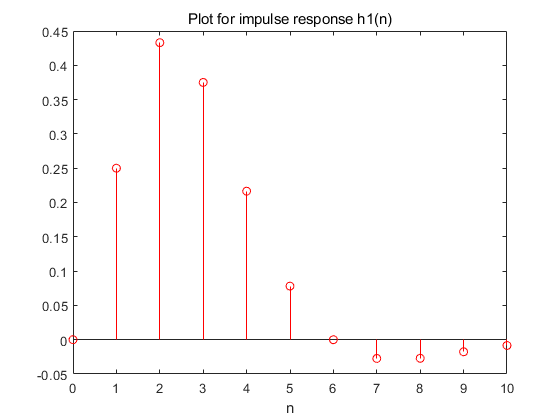
\includegraphics[width=\textwidth]{QuestionOneA.png}

(b) Using $b^{n}\sin(an) = \frac{\sin(a)bz}{z^{2}-2cos(a)bz+b^{2}}$ and $nx[n]=-z(\frac{dX(z)}{dz})$, it yields
\begin{align*}
a &= \frac{\pi}{6} \\
b &= 0.5 \\
X(z) &= \frac{0.5 \sin(\frac{\pi}{6})z}{z^{2}-2 \cos(\frac{\pi}{6}) 0.5z + 0.25} \\
&= \frac{z}{4z^2-2 \sqrt{3}z+1} \\
z\frac{dX(z)}{dz} &= z\frac{-4z^{2}+1}{(4z^{2}-2 \sqrt{3}z+1)^{2}} \\
&= \frac{-4z^{3}+z}{(4z^{2}-2 \sqrt{3}z+1)^{2}} \\
H(z) &= \frac{N(z^{-1})}{D(z^{-1})} = \frac{-4z^{3}+0z^{2}+z+0}{16z^{4}-16\sqrt{3}z^{3}+20z^{2}-4\sqrt{3}z+1} \\
H(z) &= \frac{N(z)}{D(z)} = \frac{z^{-4}(0-4z^{-1}+0z^{-2}+z^{-3}+0z^{-4})}{z^{-4}(16-16\sqrt{3}z^{-1}+20z^{-2}-4\sqrt{3}z^{-3}+z^{-4})} \\
&= \frac{0-4z^{-1}+0z^{-2}+z^{-3}+0z^{-4}}{16-16\sqrt{3}z^{-1}+20z^{-2}-4\sqrt{3}z^{-3}+z^{-4}}
\end{align*}

(c) Code and plot for $h_2[n]$
\begin{lstlisting}[language=Matlab]
x = zeros(1, 10);
x(1) = 1;
N = [-4 0 1];
D = [16 -16*sqrt(3) 20 -4*sqrt(3) 1];
h2 = filter(N, D, x);

stem(h2, 'b*');
title('Plot for h2(n)');
xlabel('n');
\end{lstlisting}

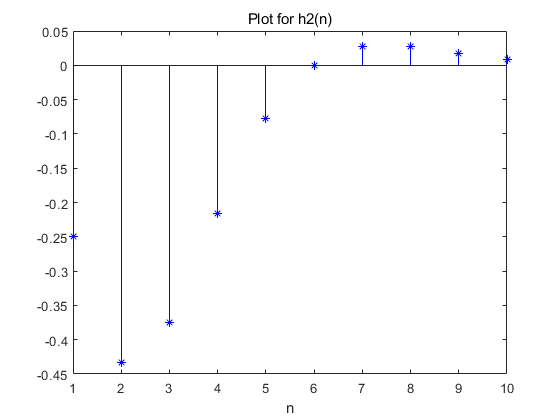
\includegraphics[width=\textwidth]{QuestionOneC.png}

(d) The value of $h_2[n]$ for each n has the same magnitude to $h_1[n]$ but with inverted sign.
\begin{lstlisting}[language=Matlab]
n = (0:1:10);
h1 = n .* 0.5 .^ n .* sin(pi / 6 .* n);

x = zeros(1, 10);
x(1) = 1;
N = [-4 0 1];
D = [16 -16*sqrt(3) 20 -4*sqrt(3) 1];
h2 = filter(N, D, x);

stem(h2, 'b*');
title('Plot for h2(n)');
xlabel('n');

stem(n, h1, 'r-');
hold on
stem(h2, 'b*');
title('h1(n) and h2(n)');
xlabel('n');
legend({'h1(n)', 'h2(n)'}, 'Location', 'southwest');
\end{lstlisting}

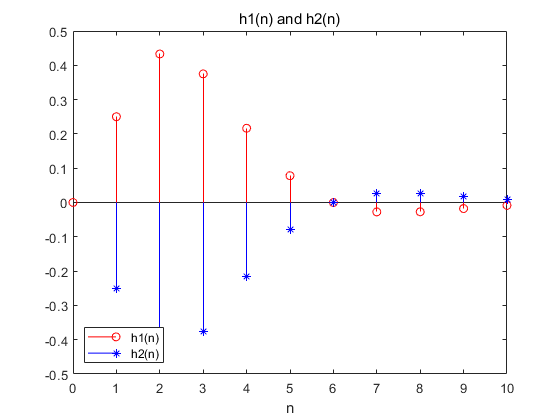
\includegraphics[width=\textwidth]{QuestionOneD.png}

\section*{Question 2}
(a) $H_1(z)$ is unstable because the only pole of $H_1(z)$, which is $z=1.25$, is outside of the unit circle $|z|=1$. $H_2(z)$ is stable because the only pole of $H_2(z)$, which is $z=0.8$, is inside of the unit circle $|z|=1$.

\begin{lstlisting}[language=Matlab]
b1 = [2 2];
a1 = [1 -1.25];
[z1, p1, k1] = tf2zpk(b1, a1);

b2 = [2 2];
a2 = [1 -0.8];
[z2, p2, k2] = tf2zpk(b2, a2);

zplane(z1, p1);
title('Pole-zero diagram for H1(z)');
xlabel('Real axis');
ylabel('Imaginary axis');

zplane(z2, p2);
title('Pole-zero diagram for H2(z)');
xlabel('Real axis');
ylabel('Imaginary axis');
\end{lstlisting}

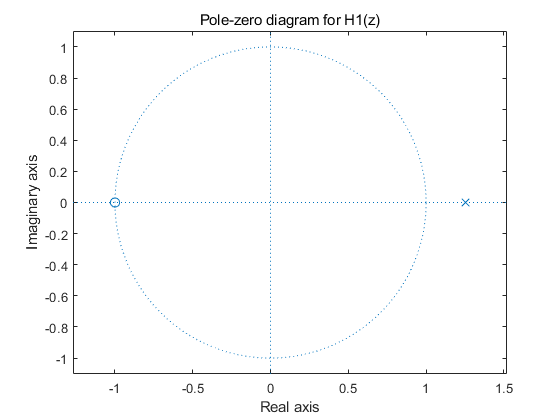
\includegraphics[width=\textwidth]{QuestionTwoA1.png}

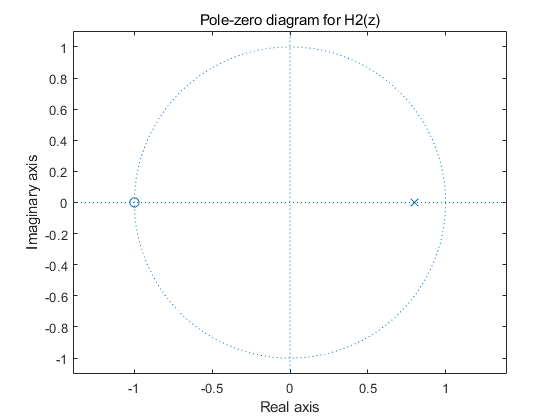
\includegraphics[width=\textwidth]{QuestionTwoA2.png}

(b) \begin{lstlisting}[language=matlab]
w = (0:0.01:2*pi());
H1 = (2 + 2 .* exp(-1j .* w)) ./ (1 - 1.25 .* exp(-1j .* w));
H2 = (2 + 2 .* exp(-1j .* w)) ./ (1 - 0.8 .* exp(-1j .* w));

magH1 = abs(H1);
magH2 = abs(H2);

phaseH1 = angle(H1);
phaseH2 = angle(H2);

%subplot(2, 1, 1);
%plot(w, magH1);
%title('Magnitude of the frequency response of H1(z)');
%xlabel('w');
%ylabel('|H1(z)|');

%subplot(2, 1, 2);
%plot(w, phaseH1);
%title('Phase of the frequency response of H1(z)');
%xlabel('w');
%ylabel('angle(H1(z))');

subplot(2, 1, 1);
plot(w, magH2);
title('Magnitude of the frequency response of H2(z)');
xlabel('w');
ylabel('|H2(z)|');

subplot(2, 1, 2);
plot(w, phaseH2);
title('Phase of the frequency response of H2(z)');
xlabel('w');
ylabel('angle(H2(z))');
\end{lstlisting}

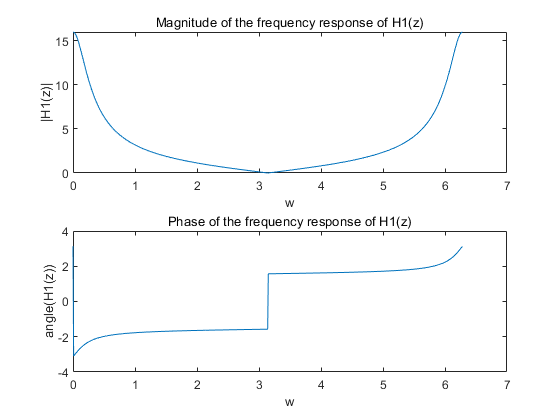
\includegraphics[width=\textwidth]{QuestionTwoB1.png}

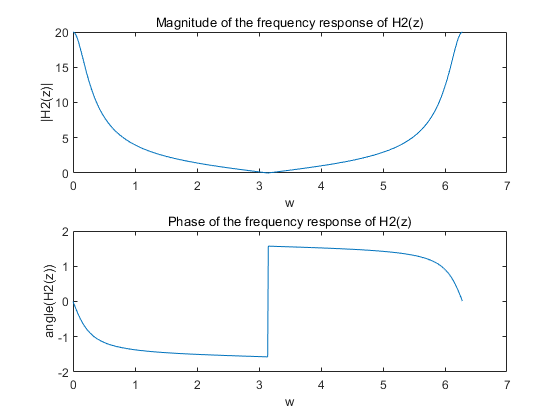
\includegraphics[width=\textwidth]{QuestionTwoB2.png}

(c) $h_1[n] = -1.6\delta[n]+3.6\cdot1.25^{n}u[n]$ and $h_2[n] = -2.5\delta[n] + 4.5\cdot0.8^{n}u[n]$.The plots in (c) matches the stability stated in part (a). $h_1[n]$ is unstable. The impulse response grows exponentially to infinity when n approaces $\inf$.$h_2[n]$ is stable. The impulse response decreases exponentially to 0 when n approaces $\inf$.

\begin{lstlisting}[language=matlab]
n = (0:25);
h1 = 3.6 * 1.25 .^ n;
h1(1) = h1(1) + -1.6;

h2 = 4.5 * 0.8 .^ n;
h2(1) = h2(1) + -2.5;

stem(n, h1);
title('Plot for impulse response h1[n]');
xlabel('n');

stem(n, h2);
title('Plot for impulse response h2[n]');
xlabel('n');
\end{lstlisting}

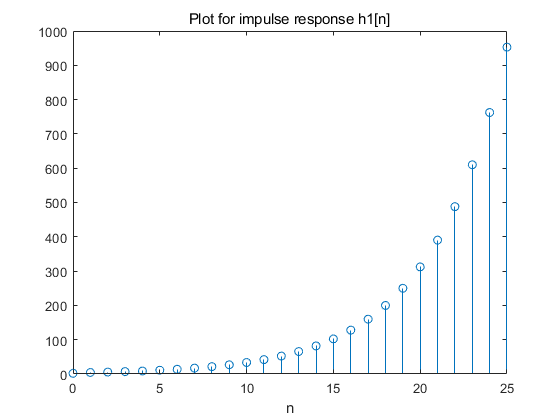
\includegraphics[width=\textwidth]{QuestionTwoC1.png}

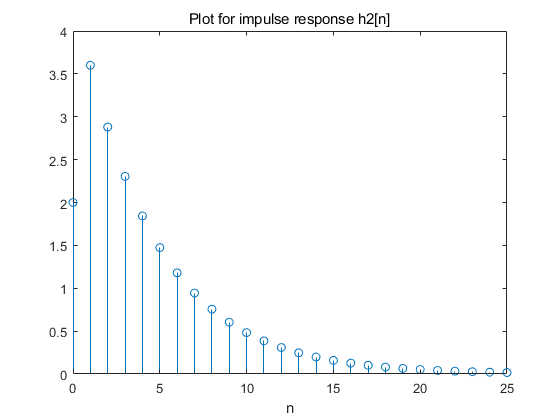
\includegraphics[width=\textwidth]{QuestionTwoC2.png}

\end{document}